\section{Simulations} \label{sec:sim}
\subsection{Methods}
We evaluate the performance of QAOA$_1$, MAQAOA$_1$, and XQAOA$_1^{\text{X=Y}}$ on max-cut instances of complete, weighted graphs, converted from randomly generated number partitioning problems. Problem ratios $0.2\leq m/n\leq 2.0$ (for $n=10$ and $2\leq m\leq 20$) and $0.5\leq m/n\leq 4.0$ (for $2\leq n\leq 16$ and $m=8$) were considered. 

For each ratio, 25 problem instances were generated. To find the expectation values for the problems, we used Equation \ref{eq:cost} alongside the analytical expressions from theorems \ref{thm:qaoa}, \ref{thm:maqaoa}, and \ref{thm:xqaoa} to find the number partitioning cost for QAOA$_1$, MAQAOA$_1$, and XQAOA$_1^{\text{X=Y}}$ respectively. We used the L-BFGS-B algorithm provided by \href{https://docs.scipy.org/doc/scipy/reference/optimize.minimize-lbfgsb.html}{\texttt{scipy.optimize.minimize}} to optimise the variational parameters for each of the algorithms that minimises the cost. Since these algorithms are heavily dependent on their initial parameters (see Section \ref{disc:ansatz}), we randomly sampled the initial parameters ($\beta\in[0,\pi]$, $\gamma\in[0,2\pi]$) 20 times and found the cost value after optimising those parameters for each problem instance, creating a distribution. We also applied the Goemans-Williamson algorithm for max-cut to our problem instances \cite{goemans1994879}, where the relaxed problem was first solved with the SCS algorithm provided by \href{https://www.cvxpy.org/tutorial/advanced/index.html}{\texttt{CVXPY}} before generating 20 random vectors for hyperplane-rounding.

We then compare the results with the classical number partitioning heuristic algorithms, greedy and Karmarkar-Karp \cite{korf2009multi}. These algorithms are deterministic and so were only needed to be run once for each problem instance. The median cost for each ratio was then compared to the distributions obtained by QAOA$_1$, MAQAOA$_1$, XQAOA$_1^{\text{X=Y}}$, and Goemans-Williamson. The results were benchmarked with the median partition difference found by using the Gurobi solver \cite{gurobi} for each problem ratio which found the optimal solution for each problem.



\subsection{Results}

Benchmarking the QAOA variants against the Goemans-Williamson, greedy, and Karmarkar-Karp algorithms, we found that the XQAOA$_1^\text{X=Y}$ variant consistently outperformed all of the other QAOA variants as well as the Goemans-Williamson algorithm for max-cut, but did worse than the classical heurstic greedy and Karmarkar-Karp algorithms. 

In the dataset with fixed $n=10$ (Figure \ref{fig:fixed_n}), we see that as $m$ increased, the median partition difference increased logarithmically for all algorithms. The boxplots reveals that the interquartile ranges of the costs of XQAOA$_1^\text{X=Y}$ is significantly lower for all problem ratios. We note that the SCS algorithm used in the Goemans-Williamson algorithm was not able to solve any problem instance for $m>11$ as the problems were unbounded.

In the dataset with fixed $m=8$ (Figure \ref{fig:fixed_m}), we see that the median costs of XQAOA$_1^\text{X=Y}$ is lower than the other variants as well as being lower than that of Goemans-Williamson for $n>3$. Figure \ref{fig:fixed_m_normal} depicts only the probabilistic plots for varying $n$ values on a linear axis. It becomes clear then that the median values for XQAOA$_1^\text{X=Y}$ remains in roughly the same range as $n$ varies with positively skewed distributions for all problem instances. The performance of QAOA$_1$ and MAQAOA$_1$ are on par with each other, but struggled with problems considered ``easy'' ($m/n <1$).

%\begin{figure}
%    \centering
%    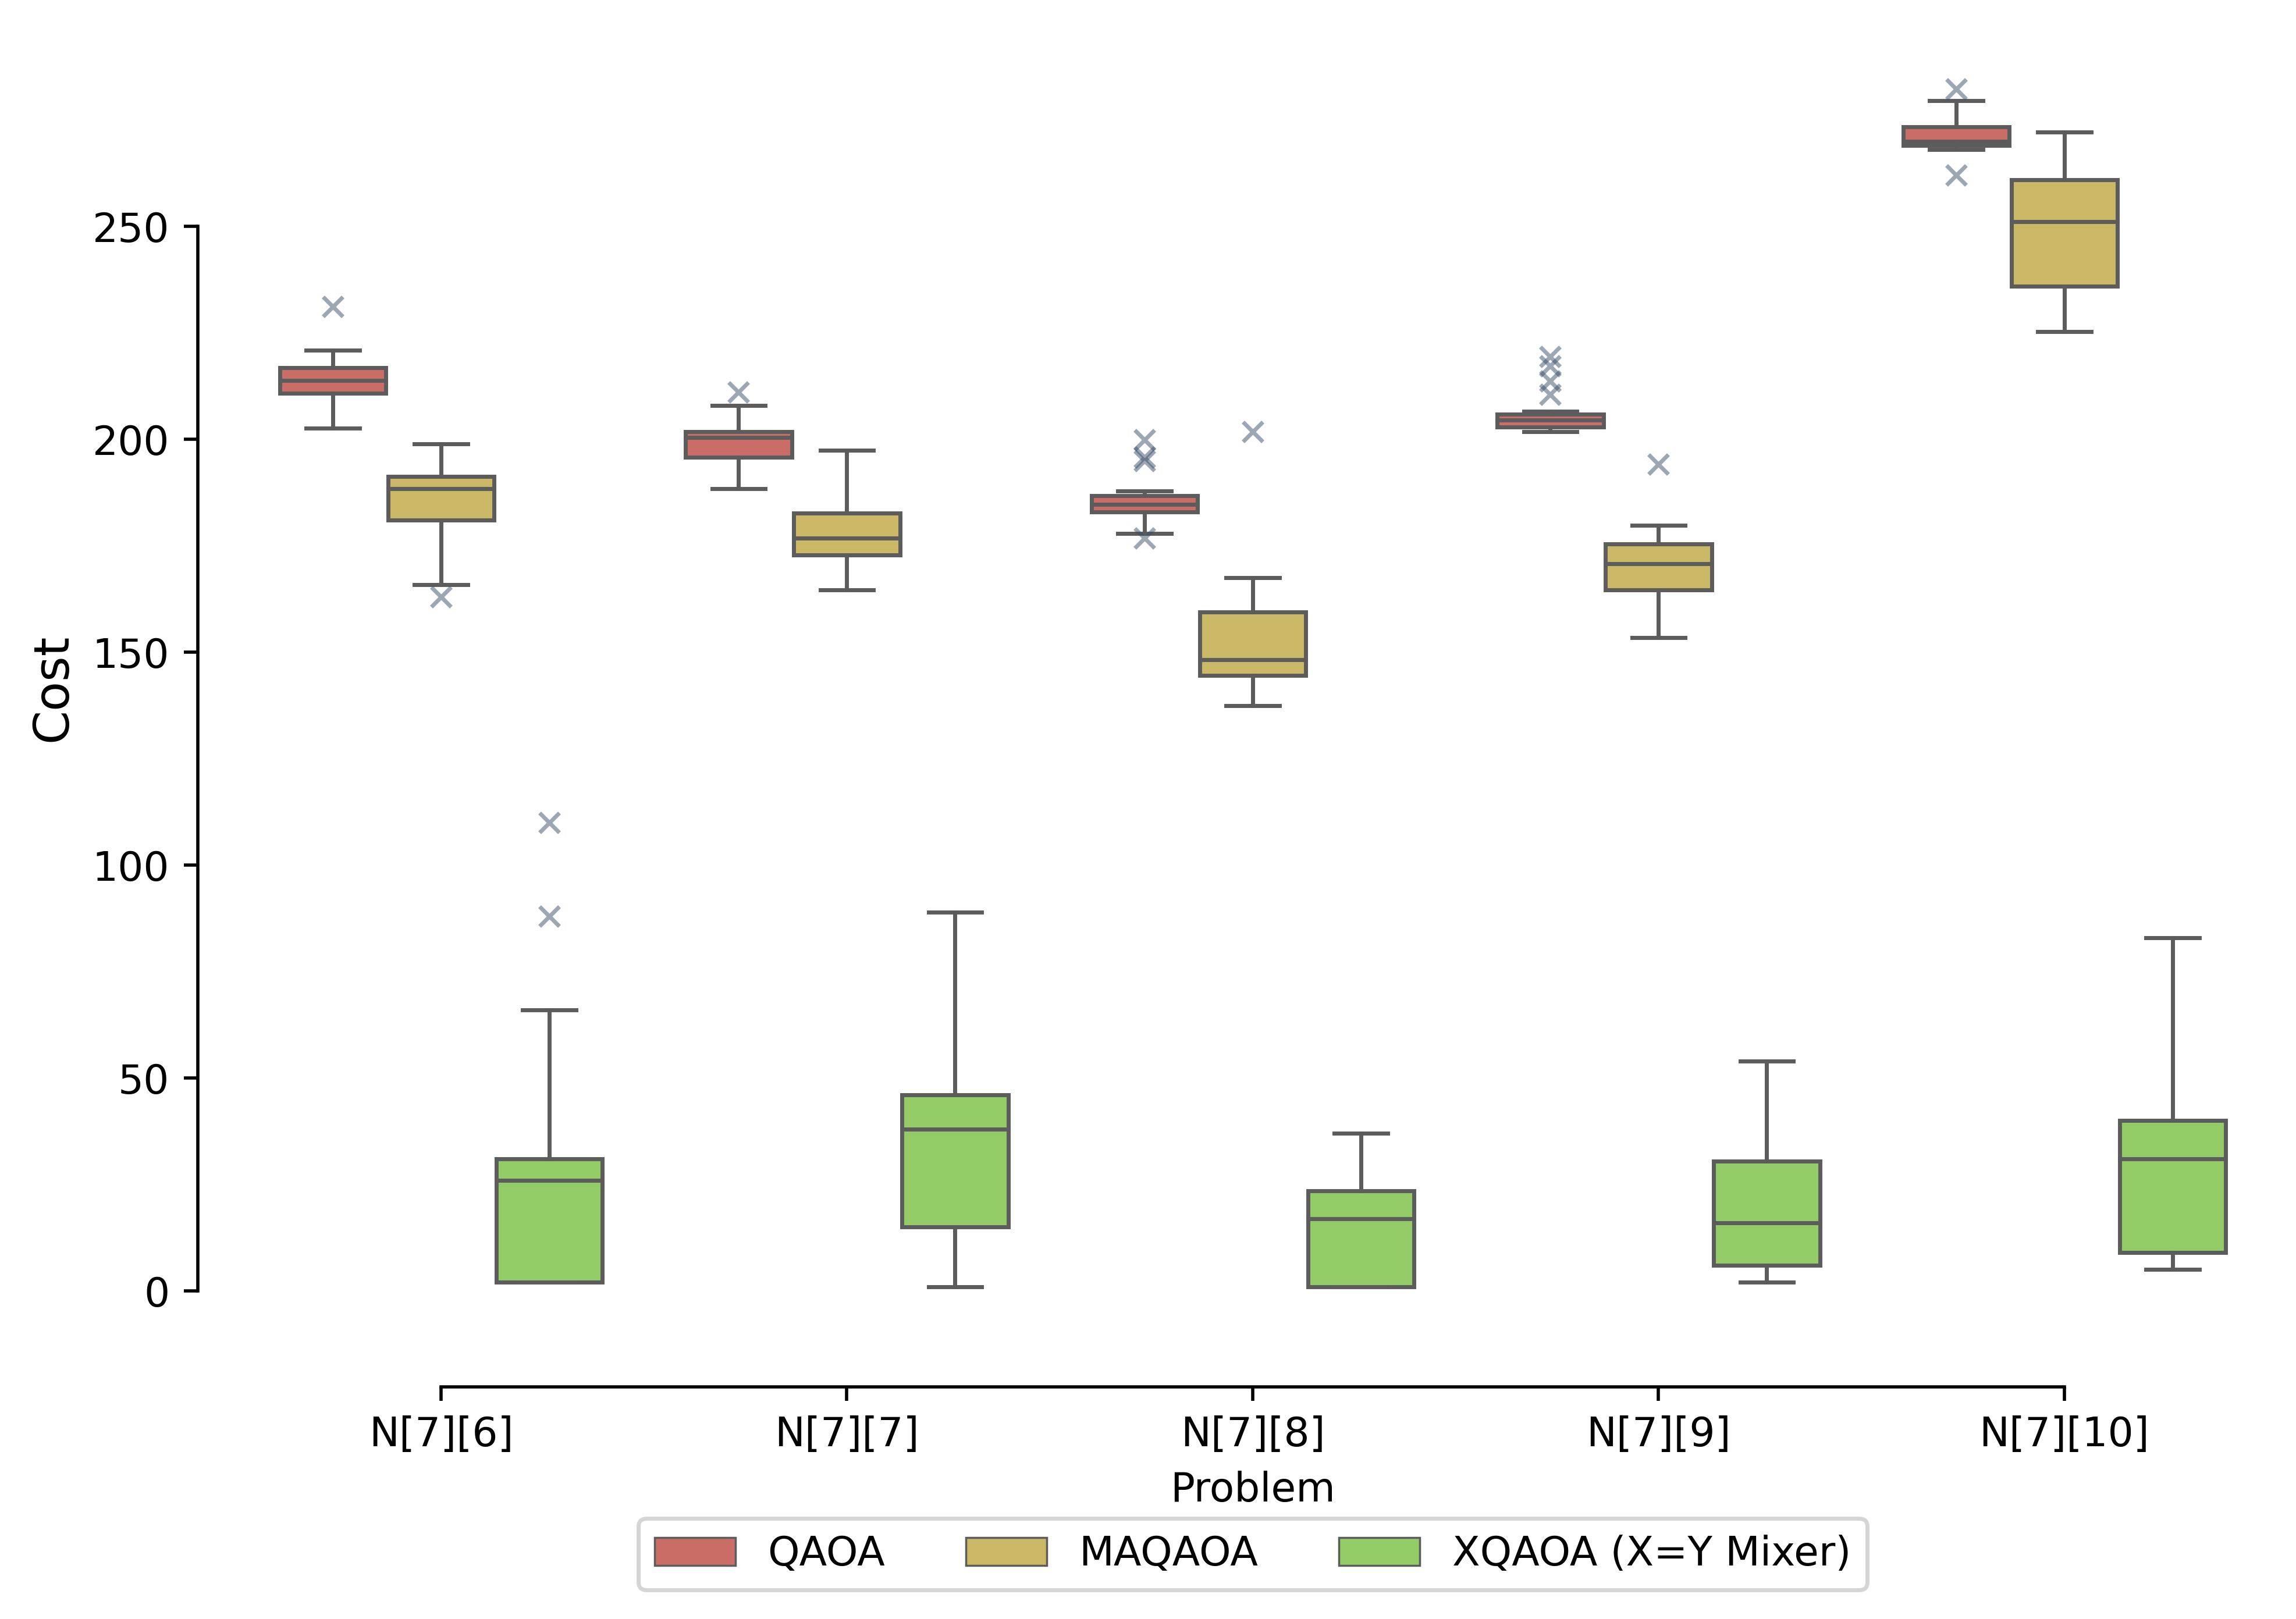
\includegraphics[scale=0.6]{"../figures/variants.png"}
%    \caption{}
%    \label{fig:variants_fixed_n_7}
%\end{figure}







